\begin{frame}{Lien entre champ de repère 2D et maillage quadrilatère}
    \begin{center}
        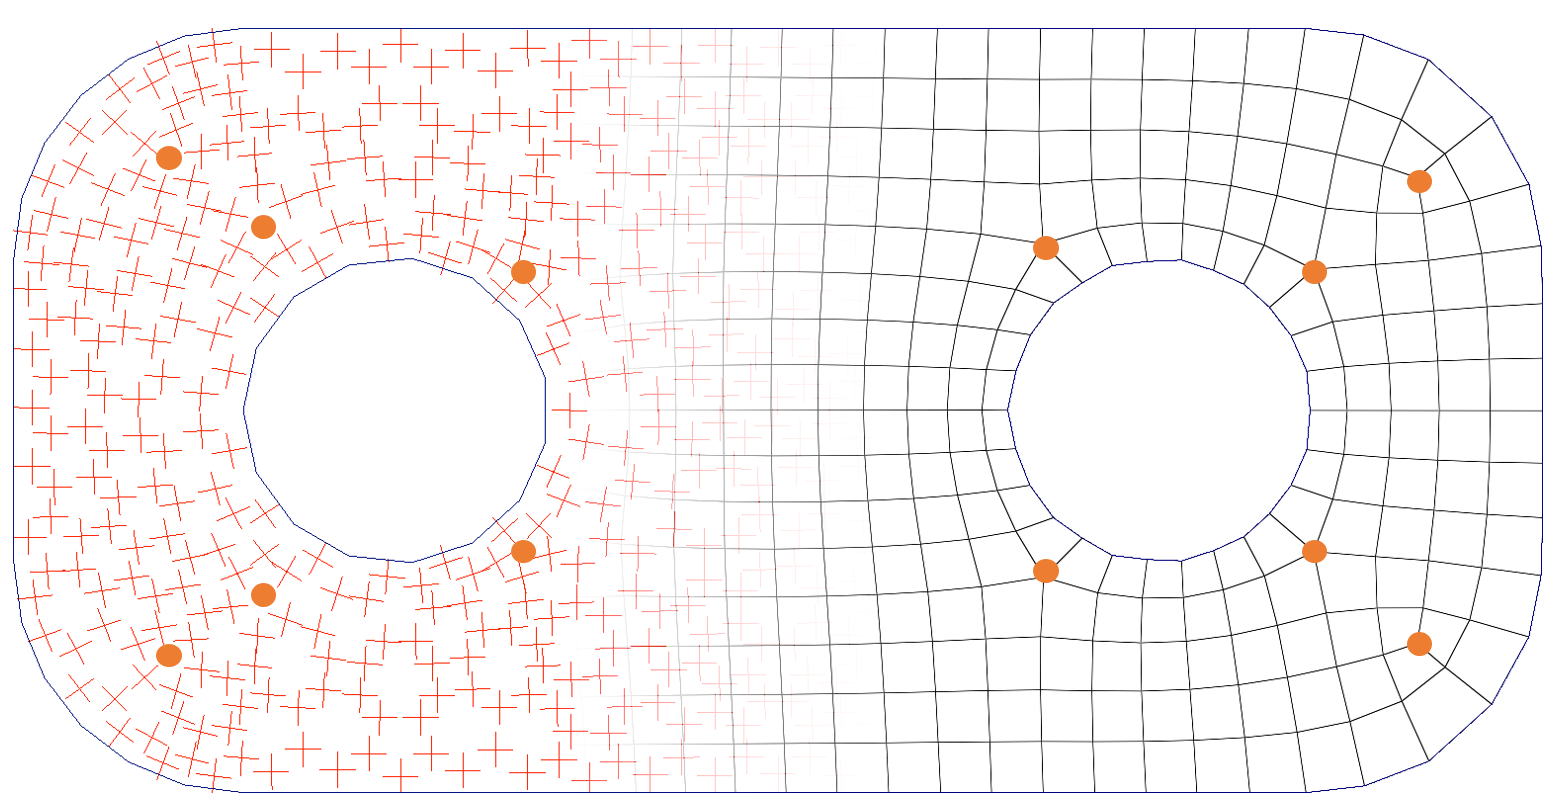
\includegraphics[width=\linewidth]{img/quadsimu/singus.PNG}
        \small{
            \textit{Les singularités d'un champ de repère sont utilisées pour déterminer la position des sommets de valence différente de 4 dans le maillage quadrilatère.}
        }
    \end{center}
\end{frame}
\begin{frame}{Quadcover pour générer un maillage quadrilatère}
    \begin{center}
        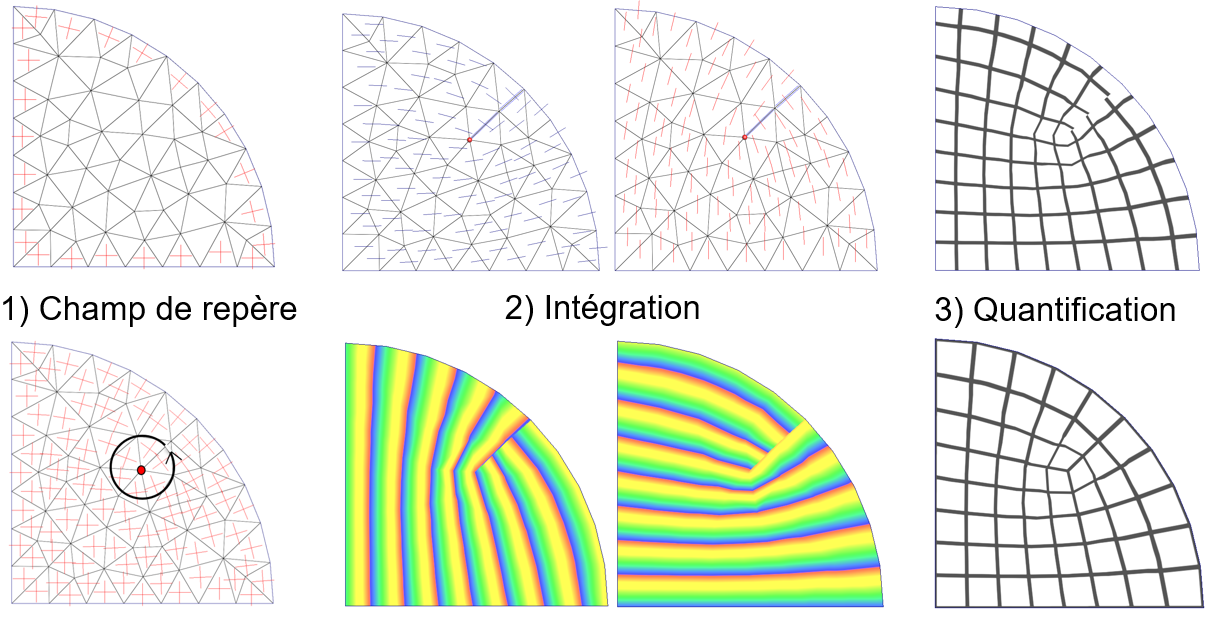
\includegraphics[width=\linewidth]{img/cubecover/pipeline.PNG}
        \small{
            \textit{Les différentes étapes de la méthode Quadcover pour construire un maillage quadrilatère.}
        }
    \end{center}
\end{frame}
\begin{frame}{En 3D: Cubecover pour générer un maillage hexaédrique}
    \begin{center}
        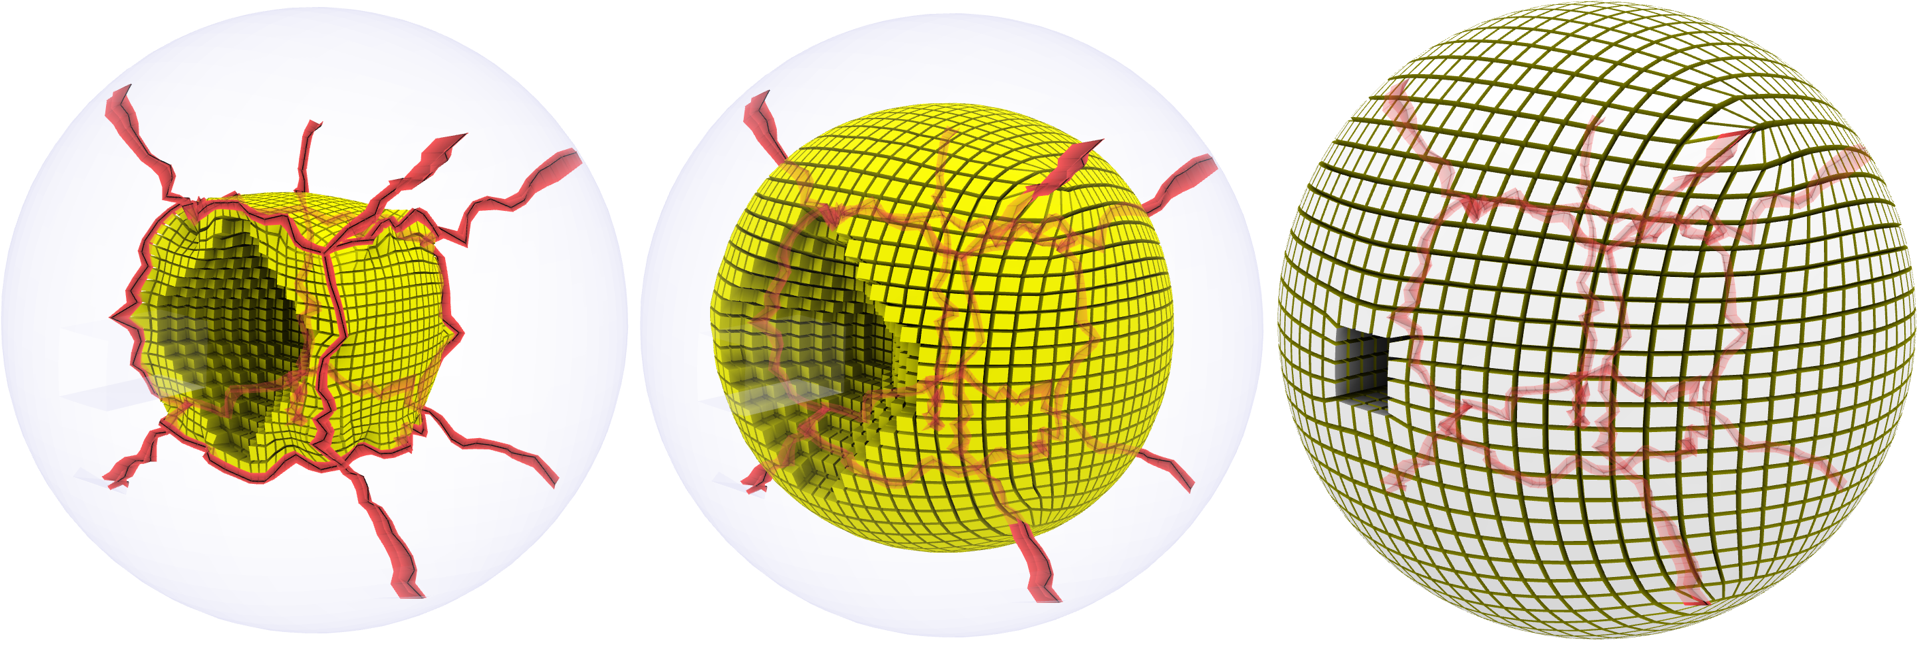
\includegraphics[width=\linewidth]{img/cubecover/B34_graphe_interieur.PNG}
        \small{
            \textit{Cubecover utilise le graphe de singularité d'un champ de repère 3D pour construire un maillage hexaédrique partageant le même graphe de singularité.}
        }
    \end{center}
\end{frame}